\documentclass[letterpaper,12pt]{article}
\usepackage[left=3cm,right=3cm,top=3cm,bottom=3cm]{geometry}
\usepackage{enumerate}
\usepackage{caption}
\usepackage{graphicx}
\usepackage{grffile}
\usepackage{float}
\usepackage[usenames]{xcolor}

\title{MATH-469 Project Checkin}
\author{Eric Biggers}

\begin{document}
\maketitle

The goal of my project is to implement an algorithm that can assemble a genome,
given a set of reads that came from it.  The key idea in the algorithm I am
implementing is the construction of a string graph where the edges are labeled
with DNA sequences and the vertices correspond to reads, and a path through the
graph corresponds to a set of reads that assemble together consistently.

I have implemented the initial stages of the algorithm.  Each step has been
implemented as a separate binary program.  This means that the overall assembly
process will iteratively transform the data (including the graph) on-disk into
the final assembly.  The main currently implemented programs are:

\begin{itemize}
%\item
	%{\tt convert-reads}:  Imports and merges a set of reads
	%into a concise binary representation.
\item
	{\tt compute-overlaps}:  Takes as input a set of reads and outputs all
	pairwise overlaps between reads of a minimum length specified by the
	{\tt --min-overlap-len} option.  The algorithm avoids a pairwise
	comparison of all reads by using a hash table to find reads sharing a
	seed.  Only exact overlaps are considered at this point.

%\item
	%{\tt print-overlaps}:  Prints a textual representation of a set of
	%overlaps, given a file containing the overlaps in binary format.

\item
	{\tt remove-contained-reads}:
	Given a set of reads and the overlaps that were computed from them,
	finds all reads that are fully contained by another read and discard
	them, along with the corresponding overlaps.  If a pair of reads is
	identical, only one copy of the read is kept.

\item
	{\tt build-directed-string-graph}:
	Given a set of reads and the overlaps that were computed from them,
	build the {\em directed} string graph that models the genome assembly.
\item
	{\tt build-bidirected-string-graph}:
	Given a set of reads and the overlaps that were computed from them,
	build the {\em bidirected} string graph that models the genome assembly.

%\item
	%{\tt print-string-graph}:
	%Prints a textual representation of a directed or bidirected string
	%graph, or prints statistics about the graph.

\item
	{\tt transitive-reduction}:
	Given a string graph, remove edges $v \to x$ where there exist edges $v
	\to w \to x$, provided that $v \to x$ is labeled by the same sequence as
	that of $v \to w$ concatenated with $w \to x$. 
	%This program currently
	%only works on directed string graphs, but the bidirected case is in
	%progress.

\item
	{\tt collapse-unbranched-paths}:
	Given a string graph, collapse chains of vertices that have in-degree 1
	and out-degree 1.
	%This program currently only works on directed string
	%graphs, but the bidirected case is in progress.

%\item
	%{\tt digraph-to-bidigraph}:
	%Convert a directed string graph into a bidirected string graph.

\end{itemize}

The modular design allows for multiple possible data flows, but a possible flow
is
%{\tt convert-reads} $\to$
{\tt compute-overlaps} $\to$ {\tt
remove-contained-reads} $\to$ {\tt build-directed-string-graph} $\to$ {\tt
transitive-reduction} $\to$ {\tt collapse-unbranched-paths} $\to$ {\tt digraph-to-bidigraph}, which will produce a
transitively-reduced, collapsed bidirected string graph produced from overlaps
between non-contained reads.

Even with the final stages not implemented, the algorithm is already very
effective when used on completely random genomes because, since there are no
spurious overlaps in a completely random genome with adequate length reads, the
transitively-reduced string graph is a chain of vertices with no branching,
which then collapses into a single edge that will be labeled with almost all the
original sequence.
%This is true even if the genome is 15 million random base pairs, given 100 bp
%reads sampled uniformly from either strand with no errors.  (Such a genome
%takes about 1 minute to assemble with maximum memory usage 1.8 GB, with the
%main time and memory bottleneck being the {\tt compute-overlaps} program).
However, genomes with repeats will produce tangled graphs that will require the
network flow and Eulerian path parts of the overall algorithm to be implemented.

What follows is an explanation of the initial stages of the algorithm on a very
simple case.  The diagram below shows a 64-base-pair ``genome'' that has had
three 32-base-pair error-free reads taken from it.  Note that the genome is
two-stranded.  {\tt A} always pairs with {\tt T} and {\tt C} always pairs with
{\tt G}, but the two strands run in opposite directions.  Reads 1 and 2 come
from the top (reverse strand), while read 3 comes from the bottom (forward
strand).  The reads are directed as shown (e.g.  read 1 begins with {\tt ACAGC},
reading from right to left, not {\tt TGAGC}).

%make out.{bi,}digraph.{pdf,dot} out.reduced.{bi,}digraph.pdf
%out.reduced.collapsed.{bi,}digraph.pdf SAMPLE_SIZE=64 USE_PIRS=false
%MIN_OVERLAP_LEN=8 READ_LEN=32 READ_SEP=12 -B
\vspace{0.5cm}
\nopagebreak

\noindent
{\tt 1.}
{\tt \color{red} $\leftarrow$TGAGCTTAAGGCTTATCTATCTTCAGACGACA$\leftarrow$ }\\
{\tt 2.}
\hspace*{2.58cm}{\tt \color{red} $\leftarrow$TTATCTATCTTCAGACGACTATTATAGCGCGG$\leftarrow$}\\
{\tt G.}
{\tt $\leftarrow$TGAGCTTAAGGCTTATCTATCTTCAGACGACTATTATAGCGCGGCCAAGACTACGCGGAGCCCC$\leftarrow$} \\
{\tt G.}
{\tt $\rightarrow$ACTCGAATTCCGAATAGATAGAAGTCTGCTGATAATATCGCGCCGGTTCTGATGCGCCTCGGGG$\rightarrow$} \\
{\tt 3.}
\hspace*{5.16cm}{\tt \color{blue} $\rightarrow$TCTGCTGATAATATCGCGCCGGTTCTGATGCG$\rightarrow$}
\vspace{0.5cm}

From looking at the above diagram, it is apparent that read 1 overlaps with read
2 by 20 base pairs, read 2 overlaps with read 3 by 20 base pairs, and read 1
overlaps with read 3 by 8 base pairs.  The task of the {\tt compute-overlaps}
program is to determine these overlaps.  Note that an overlap may match either
the forward or reverse-complement sequence.

Before building the string graph, {\tt remove-contained-reads} is run to remove
reads that are fully contained by another read.  However, there are no such
reads in this example.

Given the set of overlaps, the next step is to build the bidirected or directed
string graph.  Both these graphs are shown on the next page.  In the directed
graphs, a node $n.B$ means the beginning of read $n$, while a node $n.E$ means
the end of read $n$.  In the bidirected graphs, node $n$ simply corresponds to
read $n$.  In both the directed and bidirected graphs, the edges are labeled by
DNA sequences; however, in the drawings, only the lengths of the sequences are
shown.

Consider graph (2A), the directed string graph after transitive reduction, and
consider the walk $1.B \to 2.B \to 3.E$.  This represents a way in which reads
1, 2, and 3 assemble together consistently.  In the simplest case, all the nodes
in a path would be $E$ nodes, and this would correspond to a sequence of reads
that assemble together as they are, with no reverse-complementation.  However,
in this case, we walk from the {\em beginning} of read 1 to the {\em beginning}
of read 2, indicating that they are laid out in reverse-complement order, before
reaching the {\em end} of read 3, which is in forward order.  This
reconstruction is consistent with how the reads were actually sampled from the
genome (shown earlier).

The other component of graph (2A) produces an equivalent assembly, but it lays
out the reads in the opposite order and assembles the other strand of the
genome.

Graph (2B) is equivalent to (2A), but combines every node $n.B$ and $n.E$ into
one node $n$ to deal with the double-strandedness in a more concise manner.  The
edges are bidirected.  A bidirected edge may be traversed either way in a walk,
but if a vertex is entered through an inward head, it must be left through an
outward head, and vice versa.

Graphs (3A) and (3B) result from collapsing unbranched paths in (2A) and (2B),
respectively.  Read 2 is preceded or succeeded only by reads 1 and 3, so its
vertice(s) can be removed, and the adjacent edges can be squashed together.  As
mentioned before, this step can theoretically produce an edge labeled with
nearly the entire genome if the genome is sufficiently short or random, as in
this case.  However, in the general case, due to genomic repeats, there will be
many branches in the graph, and this needs to be taken into account by the later
stages of the algorithm (see the last page for a slightly more complicated
graph).

\newpage
\begin{tabular}{|p{0.5\textwidth}|p{0.5\textwidth}|} \hline
\centering
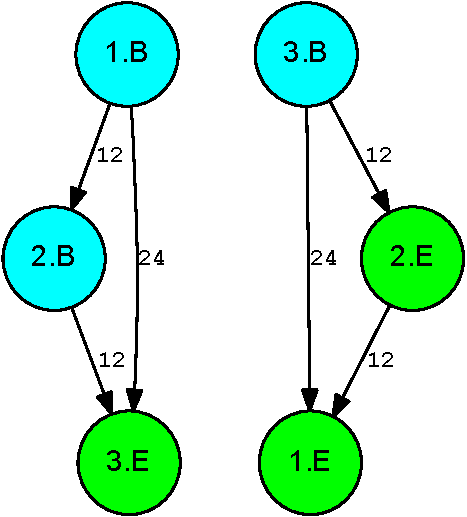
\includegraphics[scale=0.6]{out.digraph-crop.pdf}
\newline 1A. Directed string graph of original data
&
\centering
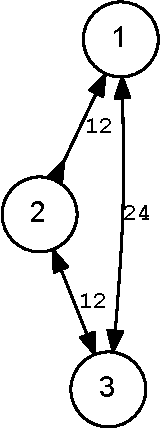
\includegraphics[scale=0.7]{out.bidigraph-crop.pdf}
\newline 1B. Equivalent bidirected string graph to (1A)
\tabularnewline \hline

\centering
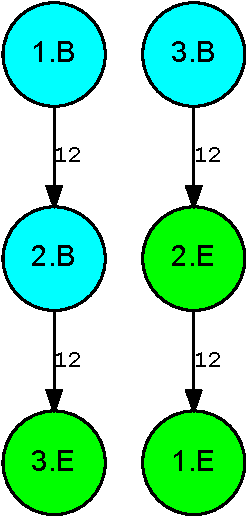
\includegraphics[scale=0.6]{out.reduced.digraph-crop.pdf}
\newline 2A. Graph (1A) after transitive reduction.  Read 2 is between reads 1
and 3, so there is no need for edges directly between 1 and 3.
&
\centering
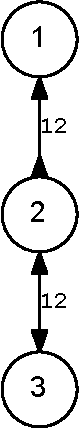
\includegraphics[scale=0.7]{out.reduced.bidigraph-crop.pdf}
\newline 2B. Graph (1B) after transitive reduction, or the equivalent bidirected
string graph to (2A)

\tabularnewline \hline

\centering
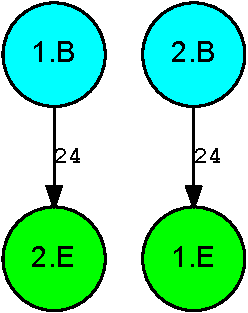
\includegraphics[scale=0.6]{out.reduced.collapsed.digraph-crop.pdf}
\newline 3A. Graph (2A) after collapsing unbranched paths
&
\centering
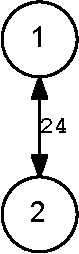
\includegraphics[scale=0.7]{out.reduced.collapsed.bidigraph-crop.pdf}
\newline 3B. Graph (2B) after collapsing unbranched paths, or the equivalent
bidirected string graph to (3A).

\tabularnewline \hline

\end{tabular}
\newpage

%make out.reduced.collapsed.{bi,}digraph.{pdf,dot} SAMPLE_SIZE=300000
%USE_PIRS=false MIN_OVERLAP_LEN=50 READ_LEN=100 READ_SEP=30 GENOME=E_coli.fa -B

\begin{figure}
\caption{Transitively-reduced, collapsed bidirected string graph for error-free
100bp reads uniformly sampled from the first 250000 base pairs of the genome of
{\it E. coli}, which includes some repetitive sequences.  The network flow
algorithm must be able to determine how many times each edge should be
traversed, then an Eulerian path through the bidirected graph must be found to
produce a possible assembly.  However, in the general case, the final
reconstruction may have to take the form of a set of paths rather than just one
path.  }
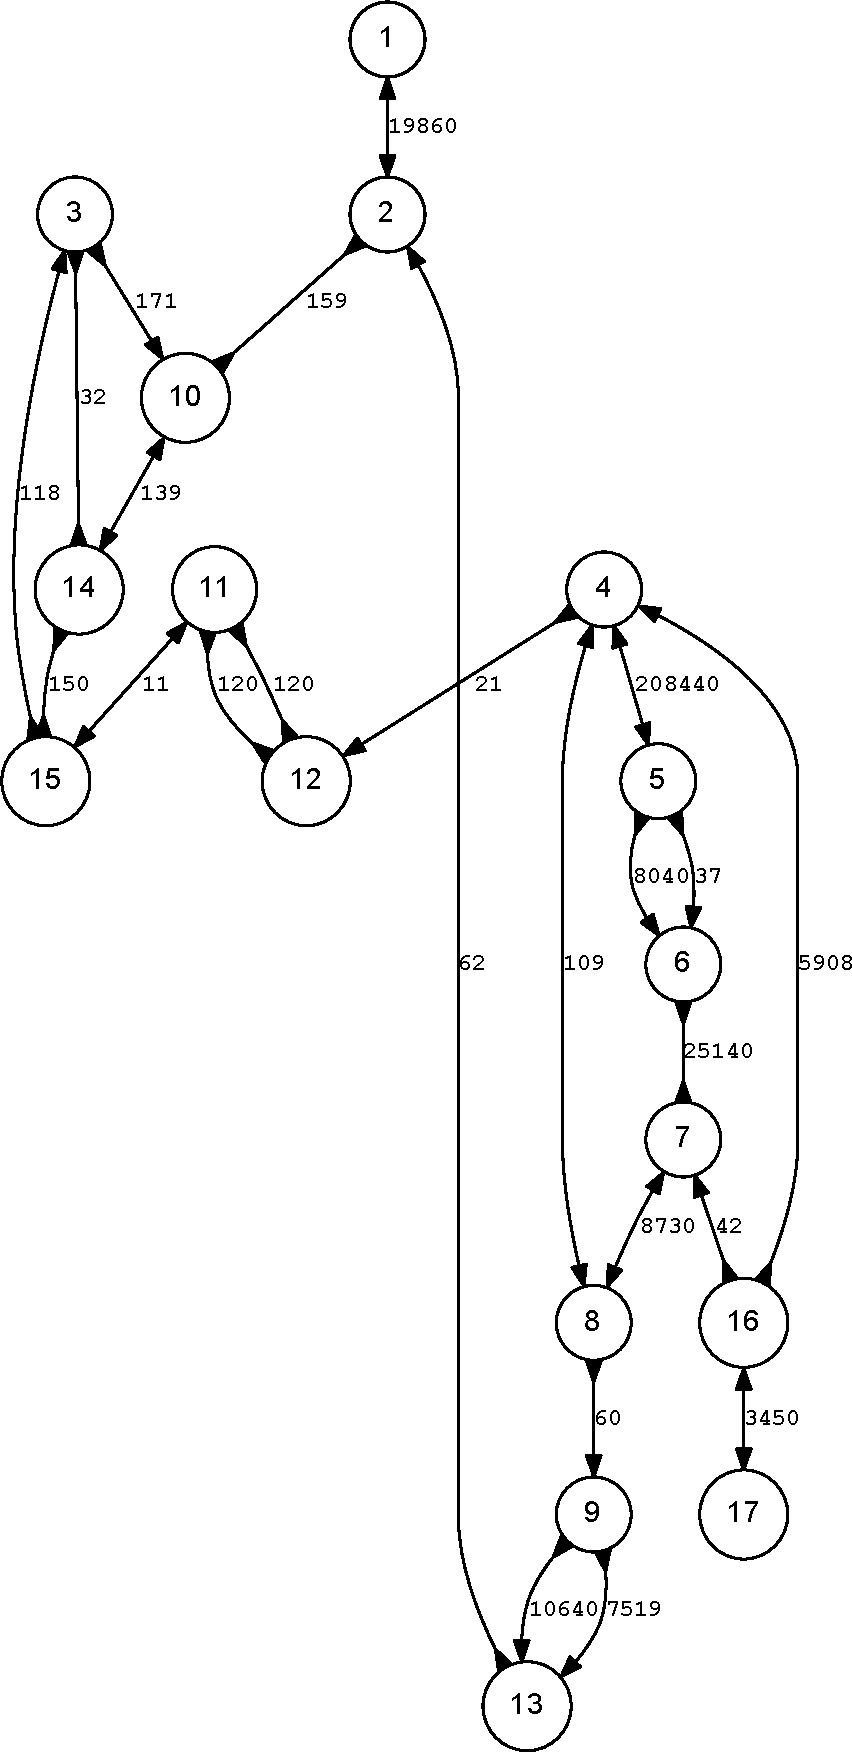
\includegraphics[scale=0.6]{E_coli-crop.pdf}
\end{figure}

\end{document}
